
\section{Techniques to tackle the problem}

Structure prediction of a dataset is a very wide topic. There are many different ways to infer the structure of a dataset. Some of the techniques include (but not limited to )

\subsection{Graph Based Semi Supervised Learning}
Graph based Semi Supervised learning first builds a graph of the dataset based on a similarity metric and then applies label propagation to infer the labels of unlabeled points.\cite{ssl1}. Figure~\ref{fig:gbssl} shows the application of the technique.

\begin{figure}[H]
	\centering
	\begin{subfigure}[t]{0.45\linewidth}
		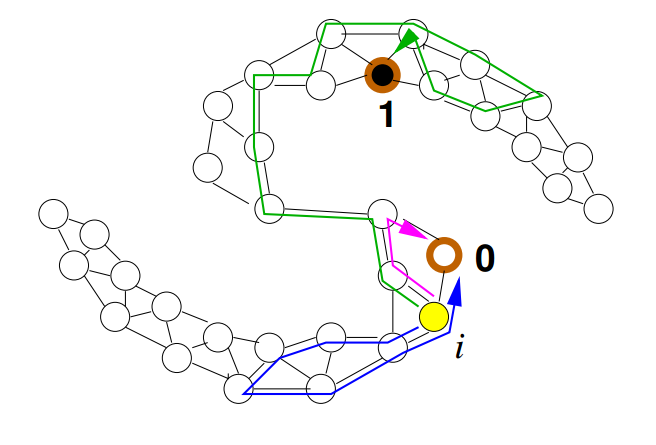
\includegraphics[width=\linewidth]{sections/imgs/techniques/gbssl1.png}
		\caption{Random Walks on Graph\cite{sslZ}}
		\label{fig:random_walk}
	\end{subfigure}
	\begin{subfigure}[t]{0.45\linewidth}
		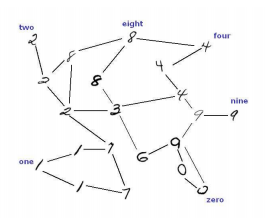
\includegraphics[width=\linewidth]{sections/imgs/techniques/gbssl2.png}
		\caption{Similarity Graph on Images\cite{ssl1}}
		\label{fig:similarity_Graph_on_images}
	\end{subfigure}
	
	\caption{Graph Based Semi Supervised Learning}
	\label{fig:gbssl}

\end{figure}

\subsection{Neural Networks}

Neural Networks can be also used to infer the structure of a dataset. They have been widely used to identify the protein secondary structure prediction \cite{protein}.
Figure \ref{fig:Protein_structure_prediction_using_neural_nets} shows an example of how a neural net might be trained to identify the structure of proteins.
\begin{figure}[H]
	%\vspace{-0.4cm}
	\centering
	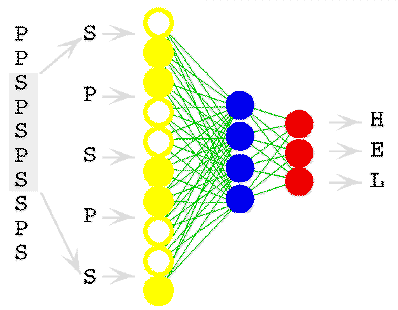
\includegraphics[width=0.5\linewidth]{sections/imgs/techniques/protein.png}
	\caption{Protein Structure Prediction using Neural Network\cite{proteinPic}}
	\label{fig:Protein_structure_prediction_using_neural_nets}
	%\vspace{-1.6cm}
\end{figure}

\subsection{Learning a Bayes Net Structure from a dataset}

Another intuitive way to identify the structure of a dataset is to learn a Bayesian Network for that data. A Bayesian network is a probabilistic graphical modelthat represents a set of random variables and their conditional dependencies via a directed acyclic graph (DAG). Figure \ref{fig:example_of_a_bayes_net} shows an example of a Bayes Net.
\begin{figure}[H]
	%\vspace{-0.4cm}
	\centering
	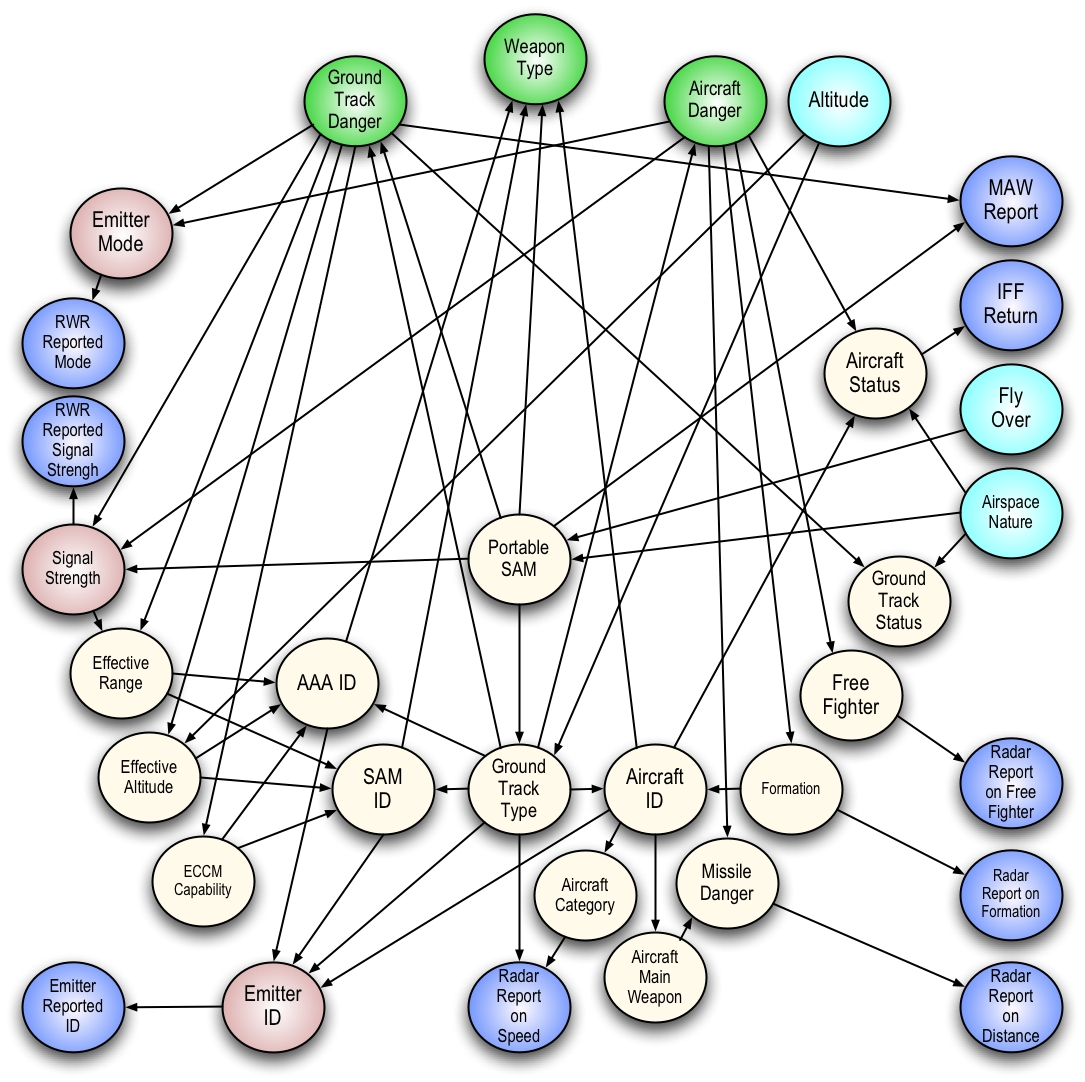
\includegraphics[width=0.5\linewidth]{sections/imgs/techniques/bnn.jpg}
	\caption{Example of an Bayesian Network\cite{bnn}}
	\label{fig:example_of_a_bayes_net}
	%\vspace{-1.6cm}
\end{figure}

\subsubsection{Different Techniques to Learn a Bayes Net}

There are three approaches to learn a Bayes Net from a data

$\bullet$ Constraint Based Structure Learning : These approaches view a Bayesian Network as a representation of independencies. They try to test out the conditional dependence and independence in the data and then try to find a network or a class of networks that best fit the data

\bigskip

$\bullet$ Score Based Structure Learning :  These approaches view the Bayesian Network as a statistical model and then address the learning problem as a model selection problem.

\bigskip

$\bullet$ Bayesian Model Averaging : This method generates an ensemble of possible structures and then averages the prediction of all the structures (similar to Bayesian Learning) 

\bigskip

In this project I explore the Score Based Learning which defines a score function that defines how well a structure matches the data. Even with a scoring function this problem is  $NP-Hard$, so certain $heuristic$ search techniques are used.
Score based methods evaluate the whole structure at once so they are less sensitive to the individual features and better at making compromises between the extent to which variables are dependent in the data and the cost of adding an edge.

For a complete dataset ( with no missing values ), the maximum likelihood score based on the Bayes Net can be used to infer the correctness of the learnt Bayes Net.
\newpage
Likelihood Score can be defined as

\begin{equation}
max{Score_L(G,D)}=max{l(\theta,G):D}
\end{equation}
where $\theta$ is the set of parameters used to define the values of the random variables in the Bayes Net.

For a general Bayes net graph the likelihood score can be written as 
\begin{equation}
{Score_L(G,D)}=M\sum_{i=1}^n I_p(X_i;Pa_{X_i})  -M\sum_{i=1}^{n}H_{P}(X_i)
\end{equation}

where $I_P$ is the mutual information between the node and its parent, $H$ is the entropy of the node and $M$ is the number of training instances.


With the above likelihood function it is possible to have overfitting because the score will increase every time we add an edge to our bayes net.

To counter this Bayesian Information Criteria is used which penalizes the amount of edges in the graph. This is done by subtracting $log(\frac{M}{2})Dim(G)$ from the likelihood function.

However the problem is still $NP-Hard$ in the space of possible structures. To help with this we only consider $Tree$ $Structured$ $Networks$. They are less susceptible to overfitting and have sparse parameterization which enables them to generalize well.

\subsubsection{Tree Structured Networks}

A network $G$ is called a Tree Structured Network if each variable $X$ has at most 1 parent.
The advantages of using a tree structured network are

$\bullet$ They can be learnt efficiently - in polynomial time

$\bullet$ They are sparse therefore avoid most overfitting problems.

$\bullet$ They also capture the most important dependencies and can provide some insight into the domain.

$\bullet$ They also provide a better baseline for approximating the distribution than the set of independent marginals of different variables.

\subsubsection{Chow Liu algorithm} 
\label{sec:chowliu}

The Chow Liu algorithm \cite{chowliu} states that the best tree-structured network can be found by minimizing the Kullback-Leibler divergence between the true distribution and the tree-structured network distribution.

\begin{equation}
KL(P(X) || T(X)) = \sum _kP(X=k) log(\frac{P(X=k)}{T(X=k)})
\end{equation}

where P(X) is the true distribution, T(X) is the tree-structured
network.

The algorithm further states that to minimize $KL(P || T)$, it suffices to find the tree network T that maximizes the sum of mutual informations
over its edges.

Mathematically,

\begin{equation}
KL(P(X) || T(X)) = \sum _kP(X=k) log(\frac{P(X=k)}{T(X=k)})=-\sum_iI(X_i,Pa_{X_i}) + \sum_iH(X_i) - H(X_1,X_2......X_N)
\label{eq:treeBnn}
\end{equation}

The second term in \ref{eq:treeBnn} does not depend on the Tree network at all. So, all that remains is to maximize the mutual information between the nodes $X_i$ and their parents.

\subsubsection{Chow Liu Algorithm using Greedy Heuristic Search}

Since from \ref{sec:chowliu} we inferred that maximizing the mutual information will minimize the $KL$ divergence, we can use the following greedy algorithm to find the undirected Bayes net graph.

$\bullet$ For each pair of vars A,B, use data to estimate P(A,B),
P(A), P(B)

$\bullet$ For each pair of vars A,B calculate mutual information

$\bullet$ Calculate the maximum spanning tree over the set of
variables, using edge weights I(A,B).

$\bullet$ Transform the resulting undirected tree to a directed one by choosing a root variable
and setting the direction of all edges to be outward from it.

Since the selection of root does not affect the log-likelihood of the tree the choice of selection of the root node does not matter.
Based on the arrows made, the Chow Liu algorithm states that the given Bayes Net will best represent the data. 

\subsubsection{Tree Augmented Naive Bayes (TAN)}
\label{sec:tan}

Naive Bayes suffers from the major drawback of not taking into account the different dependencies between the features given the label of the data.  \cite{tan} explains 
Tree Augmented Naive Bayes in which conditioned on the label we learn a bayes net graph among the different features in a dataset and then do a Bayes Net Inference to solve classification problem. 

Tree augmented naive Bayes is a semi-naive Bayesian Learning method. It relaxes the naive Bayes attribute independence assumption by employing a tree structure, in which each attribute only depends on the class and one other attribute. A maximum weighted spanning tree that maximizes the likelihood of the training data is used to perform classification. Figure \ref{fig:tan} shows TAN.

\begin{figure}[H]
	%\vspace{-0.4cm}
	\centering
	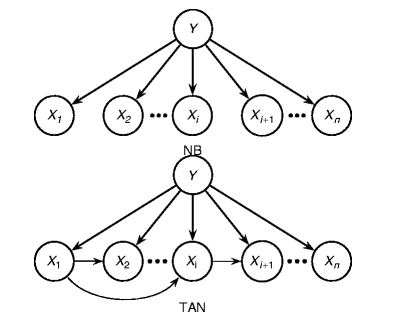
\includegraphics[width=0.4\linewidth]{sections/imgs/techniques/tan.png}
	\caption{Naive Bayes and Tree Augmented Naive Bayes\cite{tan}}
	\label{fig:tan}
	%\vspace{-1.6cm}
\end{figure}




